\documentclass[11pt,compress,t,notes=noshow, xcolor=table]{beamer}
\usepackage[]{graphicx}\usepackage[]{color}
% maxwidth is the original width if it is less than linewidth
% otherwise use linewidth (to make sure the graphics do not exceed the margin)
\makeatletter
\def\maxwidth{ %
  \ifdim\Gin@nat@width>\linewidth
    \linewidth
  \else
    \Gin@nat@width
  \fi
}
\makeatother

\definecolor{fgcolor}{rgb}{0.345, 0.345, 0.345}
\newcommand{\hlnum}[1]{\textcolor[rgb]{0.686,0.059,0.569}{#1}}%
\newcommand{\hlstr}[1]{\textcolor[rgb]{0.192,0.494,0.8}{#1}}%
\newcommand{\hlcom}[1]{\textcolor[rgb]{0.678,0.584,0.686}{\textit{#1}}}%
\newcommand{\hlopt}[1]{\textcolor[rgb]{0,0,0}{#1}}%
\newcommand{\hlstd}[1]{\textcolor[rgb]{0.345,0.345,0.345}{#1}}%
\newcommand{\hlkwa}[1]{\textcolor[rgb]{0.161,0.373,0.58}{\textbf{#1}}}%
\newcommand{\hlkwb}[1]{\textcolor[rgb]{0.69,0.353,0.396}{#1}}%
\newcommand{\hlkwc}[1]{\textcolor[rgb]{0.333,0.667,0.333}{#1}}%
\newcommand{\hlkwd}[1]{\textcolor[rgb]{0.737,0.353,0.396}{\textbf{#1}}}%
\let\hlipl\hlkwb

\usepackage{framed}
\makeatletter
\newenvironment{kframe}{%
 \def\at@end@of@kframe{}%
 \ifinner\ifhmode%
  \def\at@end@of@kframe{\end{minipage}}%
  \begin{minipage}{\columnwidth}%
 \fi\fi%
 \def\FrameCommand##1{\hskip\@totalleftmargin \hskip-\fboxsep
 \colorbox{shadecolor}{##1}\hskip-\fboxsep
     % There is no \\@totalrightmargin, so:
     \hskip-\linewidth \hskip-\@totalleftmargin \hskip\columnwidth}%
 \MakeFramed {\advance\hsize-\width
   \@totalleftmargin\z@ \linewidth\hsize
   \@setminipage}}%
 {\par\unskip\endMakeFramed%
 \at@end@of@kframe}
\makeatother

\definecolor{shadecolor}{rgb}{.97, .97, .97}
\definecolor{messagecolor}{rgb}{0, 0, 0}
\definecolor{warningcolor}{rgb}{1, 0, 1}
\definecolor{errorcolor}{rgb}{1, 0, 0}
\newenvironment{knitrout}{}{} % an empty environment to be redefined in TeX

\usepackage{alltt}
\newcommand{\SweaveOpts}[1]{}  % do not interfere with LaTeX
\newcommand{\SweaveInput}[1]{} % because they are not real TeX commands
\newcommand{\Sexpr}[1]{}       % will only be parsed by R



\usepackage[english]{babel}
\usepackage[utf8]{inputenc}

\usepackage{dsfont}
\usepackage{verbatim}
\usepackage{amsmath}
\usepackage{amsfonts}
\usepackage{bm}
\usepackage{csquotes}
\usepackage{multirow}
\usepackage{longtable}
\usepackage{booktabs}
\usepackage{enumerate}
\usepackage[absolute,overlay]{textpos}
\usepackage{psfrag}
\usepackage{algorithm}
\usepackage{algpseudocode}
\usepackage{eqnarray}
\usepackage{arydshln}
\usepackage{tabularx}
\usepackage{placeins}
\usepackage{tikz}
\usepackage{setspace}
\usepackage{colortbl}
\usepackage{mathtools}
\usepackage{wrapfig}
\usepackage{bm}
\usetikzlibrary{shapes,arrows,automata,positioning,calc,chains,trees, shadows}
\tikzset{
  %Define standard arrow tip
  >=stealth',
  %Define style for boxes
  punkt/.style={
    rectangle,
    rounded corners,
    draw=black, very thick,
    text width=6.5em,
    minimum height=2em,
    text centered},
  % Define arrow style
  pil/.style={
    ->,
    thick,
    shorten <=2pt,
    shorten >=2pt,}
}
\usepackage{subfig}


% Defines macros and environments
\input{../../style/common.tex}

%\usetheme{lmu-lecture}
\newcommand{\titlefigure}{figure_man/intro-titlefig.jpg}
\newcommand{\learninggoals}{
\item Understand the goal of performance estimation
\item Know the definition of generalization error
\item Understand the difference between outer and inner loss}
\usepackage{../../style/lmu-lecture}

\let\code=\texttt
\let\proglang=\textsf

\setkeys{Gin}{width=0.9\textwidth}

\title{Introduction to Machine Learning}
% \author{Bernd Bischl, Christoph Molnar, Daniel Schalk, Fabian Scheipl}
\institute{\href{https://compstat-lmu.github.io/lecture_i2ml/}{compstat-lmu.github.io/lecture\_i2ml}}
\date{}

\setbeamertemplate{frametitle}{\expandafter\uppercase\expandafter\insertframetitle}


\begin{document}


% This file loads R packages, configures knitr options and sets preamble.Rnw as parent file
% IF YOU MODIFY THIS, PLZ ALSO MODIFY setup.Rmd ACCORDINGLY...


% Defines macros and environments
\input{../../latex-math/basic-math.tex}
\input{../../latex-math/basic-ml.tex}
\input{../../latex-math/ml-automl.tex}
%! includes: basics-learners 

\lecturechapter{Evaluation: Introduction and Remarks}
\lecture{Introduction to Machine Learning}

% ------------------------------------------------------------------------------

\begin{vbframe}{Performance estimation}

\begin{itemize}
  \item After training our model, we are naturally interested in its
  \textbf{performance}.
  \item We recall what supervised learning is about: 
  
  $$\inducer: \preimageInducerShort \rightarrow \Hspace, \quad (\D, \lambdav)
  \mapsto \fh_{\D, \lambdav}$$
  \item $\inducer$ minimizes the empirical risk resulting from $\Lyf$.
  \item This so-called \textbf{inner loss}, however, is only a statistical proxy
  to what we are really interested in: the \textbf{true expected loss} for 
  new, unlabeled data.
  \item After all, we chose our model precisely so it would be loss-minimal 
  on the data we trained it on, but we cannot hope for it to perform equally 
  well on general data from $\Pxy$.
\end{itemize}

\lz
$\rightarrow$ Evaluation based on the inner loss would be 
\textbf{optimistically biased}.

\end{vbframe}

% ------------------------------------------------------------------------------

\begin{vbframe}{Generalization error}

\begin{itemize}
  \item The true expected loss for a model $\fh_{\D_n, \lambdav}$, learned on 
  $\D_n \sim \Pxy$, is measured w.r.t. to previously 
  unseen data $(\xv, y) \sim \Pxy$.
  \item We refer to this as \textbf{generalization error} or \textbf{outer 
  loss}:
  $$\mathrm{GE}(\fh_{\D_n, \lambdav}) := \E_{(\xv, y) \sim \Pxy}\left[ 
  L\left(y, \fh_{\D_n, \lambdav}(\xv)\right) \right]$$
  \item The goal of \textbf{performance evaluation} is to measure 
  $\mathrm{GE}(\fh_{\D_n, \lambdav})$. \\
  $\rightarrow$ As $\Pxy$ is unknown to us, we can only estimate it.
\end{itemize}

\begin{center}
% FIGURE SOURCE: https://docs.google.com/drawings/d/13AH298rMnDL5p0SrBd6VCukC9vg1qyRXGqgMcvuPRc0/edit?usp=sharing
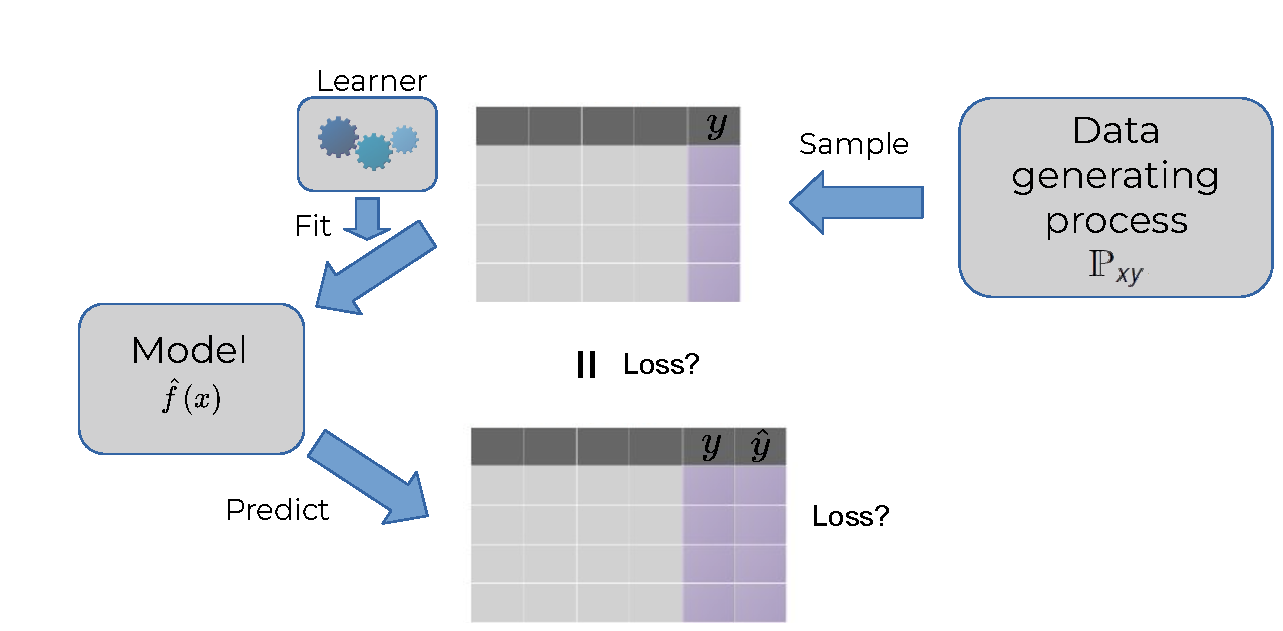
\includegraphics[width=0.6\textwidth]{figure_man/evaluation-intro-ge.pdf}

\end{center}

\end{vbframe}

% ------------------------------------------------------------------------------

\begin{vbframe}{Inner vs outer loss}

\begin{itemize}
  \item Supervised learning thus implies the following dichotomy:
  \begin{itemize}
    \item \textbf{Learning}: train $\fh_{\D_n, \lambdav}$ minimizing 
    \textit{inner} loss
    \item \textbf{Evaluation}: evaluate $\fh_{\D_n, \lambdav}$ estimating
    \textit{outer} loss
  \end{itemize}
  \item Beyond evaluating a single learner, the outer loss lends itself to
  comparing different types of learners, or learners with varying hyperparameter
  configurations $\lambdav$.
\end{itemize}

\lz

\begin{itemize}
  \item Ideally, we have \textbf{inner loss = outer loss}.
  \item This is not always possible -- sometimes we use losses that are 
  hard to optimize or do not even specify one directly, as in:
  \begin{itemize}
    \item Logistic regression: minimization of binomial loss
    \item k-NN: no explicit loss minimization
  \end{itemize}
  \item On the other hand, there are some special metrics for evaluation,
  such as those derived from ROC curves.
\end{itemize}

\end{vbframe}

% ------------------------------------------------------------------------------

\begin{vbframe}{Inner vs outer loss}

\small

\textbf{Example:} logistic regression

\begin{itemize}
  \item An intuitive choice for the loss in logistic regression would be to
  evaluate the share of incorrect predictions.
  \item This leads to the \textbf{mislassification error rate (MCE)}, computing
  the mean over pointwise \textbf{0-1 loss}.
\end{itemize}

\lz

\begin{minipage}{0.6\textwidth}
  \begin{itemize}
    \item 0-1 loss simply assigns a loss of 1 for incorrect predictions and 0
    otherwise: $$\Lhxy = [y - \hx]$$
  \end{itemize}
\end{minipage}%
\begin{minipage}{0.4\textwidth}
  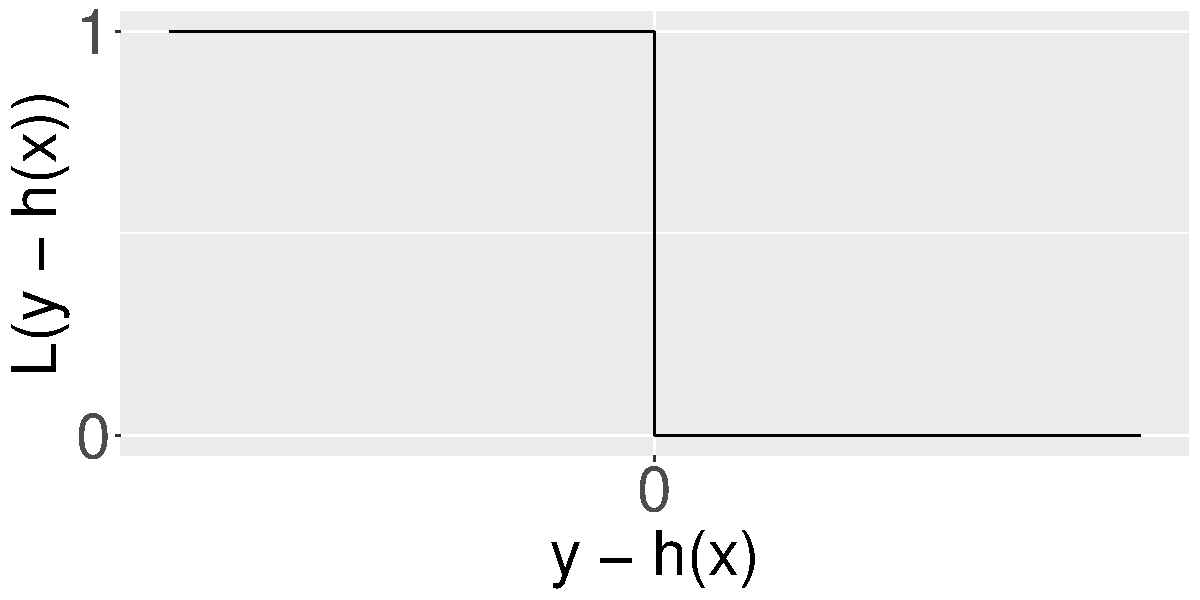
\includegraphics[width=0.8\textwidth]{figure/zero-one-loss}
\end{minipage}

\lz

\begin{itemize}
  \item Problem: 0-1 loss is not differentiable (not continuous even). \\
  $\rightarrow$ This is why we use binomial loss as \textbf{inner} loss 
  instead.
  \item For evaluation, differentiability is not required. \\
  $\rightarrow$ We may use 0-1 as \textbf{outer} loss and evaluate our 
  learner on its MCE. 
\end{itemize}

\normalsize

\end{vbframe}

% ------------------------------------------------------------------------------

\begin{vbframe}{Training and test data}

\begin{itemize}
  \item For reliable estimates of $\mathrm{GE}(\fh_{\D_n, \lambdav})$ we need 
  \textbf{test data} that are independent of the data we trained our model on.
  \item Such test sets are not always available, but we will learn about 
  techniques of \textbf{resampling} that allow us to carve out test sets from 
  the data at hand.
\end{itemize}

\begin{center}
  % FIGURE SOURCE: https://docs.google.com/presentation/d/1CDxKPNn2J7oZQOY62mlXS-s4Bu0IUiw57cjfCXOpzDk/edit#slide=id.p
  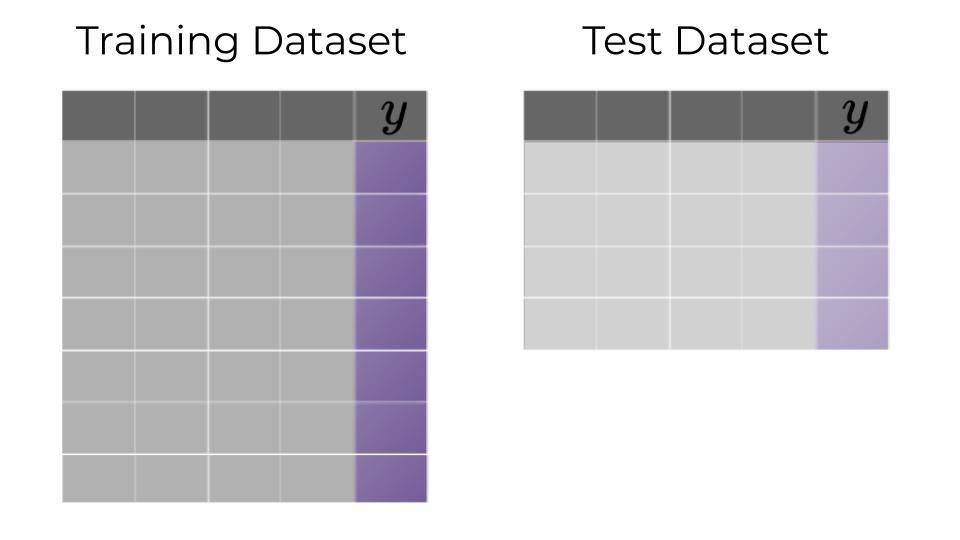
\includegraphics[width=0.4\textwidth]{figure_man/train-test-data.jpg}
\end{center}

\begin{itemize}
  \item Note that this paradigm is somewhat different from traditional 
  statistical model diagnosis where models are judged by their goodness-of-fit 
  rather than their generalization ability.
  % \item The goodness-of-fit measures employed there (such as $R^2$ or 
  % information criteria) are rooted in regression modeling and are based, in a
  % broad sense, on the inner loss.
\end{itemize}

\end{vbframe}

% ------------------------------------------------------------------------------

\endlecture
\end{document}
